% This LaTeX was auto-generated from MATLAB code.
% To make changes, update the MATLAB code and export to LaTeX again.

\documentclass{article}


\usepackage[utf8]{inputenc}
\usepackage[T1]{fontenc}
\usepackage{lmodern}
\usepackage{graphicx}
\usepackage{color}
\usepackage{listings}
\usepackage{hyperref}
\usepackage{amsmath}
\usepackage{amsfonts}
\usepackage{epstopdf}
\usepackage{matlab}

\graphicspath{ {./} }

\sloppy
\epstopdfsetup{outdir=./}
%\graphicspath{ {./homework1_images/} }


\begin{document}

\matlabtitle{Empirical Methods Homework 1}
\matlabheading{Carlos Rangel}

\matlabheading{Question 1:}

\begin{par}
\begin{flushleft}
Code:
\end{flushleft}
\end{par}

\begin{matlabcode}
% Define vector X
x=[1, 1.5, 3, 4, 5, 7, 9, 10];

% Compute The Values for y1=-2 + 0.5x
y1=-2 + 0.5.*x;

% Display y1
disp(y1')
\end{matlabcode}
\begin{matlaboutput}
   -1.5000
   -1.2500
   -0.5000
         0
    0.5000
    1.5000
    2.5000
    3.0000
\end{matlaboutput}
\begin{matlabcode}
% Compute the values for y2
y2= -2 + 0.5 .* x.^2;

% Display y2
disp(y2')
\end{matlabcode}
\begin{matlaboutput}
   -1.5000
   -0.8750
    2.5000
    6.0000
   10.5000
   22.5000
   38.5000
   48.0000
\end{matlaboutput}

\newpage

\begin{matlabcode}

% Plot Y1, Y2 vs X
figure
plot(x, y1, x, y2)
title("Y1,Y2 vs. X")
xlabel("x")
legend("Y1", "Y2")
\end{matlabcode}
%\begin{center}
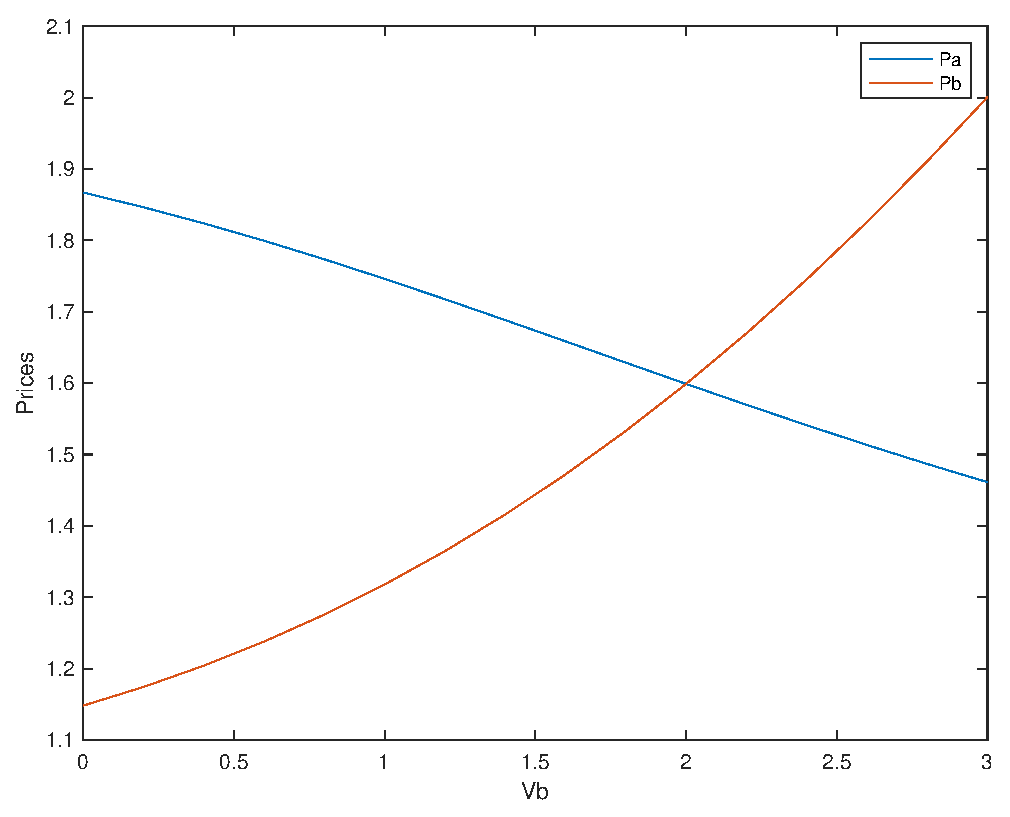
\includegraphics[width=\maxwidth{56.196688409433015em}]{figure_0}
%\end{center}


\matlabheading{Question 2}

\begin{par}
\begin{flushleft}
Code:
\end{flushleft}
\end{par}

\begin{matlabcode}
% Create x vector
x=linspace(-10, 20);

% Calculate and display sum of the elements of x
sum_x=sum(x)
\end{matlabcode}
\begin{matlaboutput}
sum_x = 500.0000
\end{matlaboutput}


\matlabheading{Question 3}

\begin{par}
\begin{flushleft}
Code:
\end{flushleft}
\end{par}

\begin{matlabcode}
% Create A matrix
A=[2, 4, 6; 1, 7, 5; 3, 12, 4];

% Create vector b
b=[-2;3;10];

% Calculate and display C=A'b
C=A'*b;

% Calculate and display D=((A'A)^(-1))*b
D=inv(A'*A)*b
\end{matlabcode}
\begin{matlaboutput}
D = 3x1    
   -3.2505
    0.3961
    0.8037

\end{matlaboutput}
\begin{matlabcode}

% Calculate and Display E= sum_i (sum_j aij*bi)
E=sum(sum(A.*b))
\end{matlabcode}
\begin{matlaboutput}
E = 205
\end{matlaboutput}
\begin{matlabcode}

% F matrix is matrix with the 2nd row and 3rd column deleted

% Initialize F to A
F=A;

% Delete 2nd row
F(2,:) = [];

% Delete 3rd column and display F
F(:,3)=[]
\end{matlabcode}
\begin{matlaboutput}
F = 2x2    
     2     4
     3    12
\end{matlaboutput}
\newpage
\begin{matlabcode}
% Solve the system Ax=b
x=A\b
\end{matlabcode}
\begin{matlaboutput}
x = 3x1    
   -0.1622
    1.2432
   -1.1081

\end{matlaboutput}


\matlabheading{Question 4}

\begin{par}
\begin{flushleft}
Code:
\end{flushleft}
\end{par}

\begin{matlabcode}
% Create block diagonal matrix

% Initialize B to a 15 x 15 zero matrix
B=blkdiag(A,A,A,A,A)
\end{matlabcode}

\includegraphics[scale=0.3]{blockmatrix}

%\begin{figure}
%	\centering
%	\subfloat[BlockMatrix]{\includegraphics[height=2.2in, width=2.9in]{blockmatrix.png}}
%\end{figure}


\matlabheading{Question 5}

\begin{par}
\begin{flushleft}
Code:
\end{flushleft}
\end{par}

\begin{matlabcode}
% Create 5x3 matrix of randome distributions with mu= 10 and std=5

A=10+5*randn(5,3)
\end{matlabcode}
\begin{matlaboutput}
A = 5x3    
    6.9984   -0.6918   10.6202
   12.4498    5.8021   17.1835
   13.6968   16.7730    0.1955
   18.5594    4.6392    9.0115
    9.0294   14.8048    3.9608

\end{matlaboutput}
\begin{matlabcode}

% Replace the elements of A that are less than 10 with 0
A(A<10)=0;

% Replace the elements of A that are equal or greater tan 10 with 1
A(A>=10)=1
\end{matlabcode}
\begin{matlaboutput}
A = 5x3    
     0     0     1
     1     0     1
     1     1     0
     1     0     0
     0     1     0

\end{matlaboutput}


\matlabheading{Question 6}

\begin{par}
\begin{flushleft}
Code:
\end{flushleft}
\end{par}

\begin{matlabcode}
% Import CSV file
data = csvread('datahw1.csv');

T=readtable('datahw1.csv', 'ReadVariableNames', false);

% Modify variable names
T.Properties.VariableNames = {'FirmID', 'Year', 'Export', 'RD', 'prod', 'cap'}

fitlm(T,'prod~Export+RD+cap')
\end{matlabcode}

\includegraphics[scale=0.3]{regression}

\end{document}
